\documentclass{article}
\usepackage{wrapfig}
\usepackage{graphicx}
\usepackage{amsmath}
\usepackage[margin=0.8in]{geometry}
\usepackage{listings}
\usepackage{float}
\usepackage[inline]{enumitem}

\setlength\intextsep{0pt}

\setlist[itemize]{noitemsep, topsep=0pt}

\title{EE2703: Assignment 5}
\author{Sakthi Harish D T (EE19B054)}
\date{March 23, 2021}


\begin{document}	
	
\maketitle {\hspace{5 cm}\textbf{Laplace Equation: Resistor problem}}	

  \section{Abstract}
  In this report we wish to discuss about,\newline
  \begin{itemize}
      \item the distribution of potential over a resistor( a copper plate) \newline
      \item solving for the currents in the resistor\newline
      \item finding the hottest part of the resistor\newline
      \item analyse the errors using semilog and loglog plots \newline
      \item using Least Squares to model the errors \newline
      \item stopping condition after analysing the errors \newline
  \end{itemize}

  \section{Introduction}
	\begin{wrapfigure}{l}{0.5\textwidth}
\centering
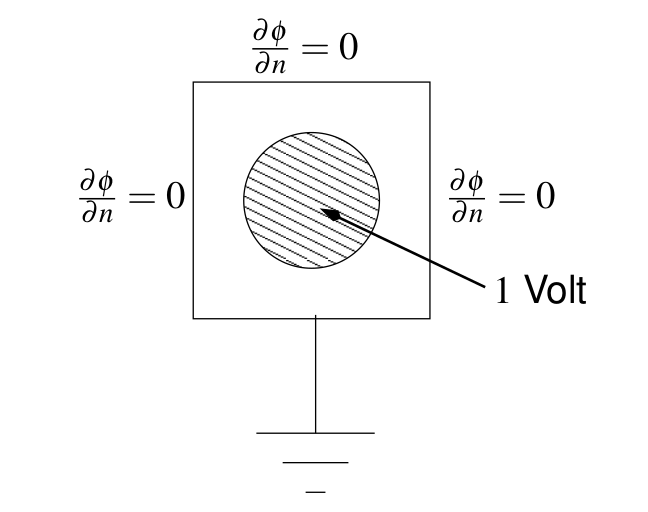
\includegraphics[width=.98\linewidth]{plateimage.png}
\caption{The copper plate}
\end{wrapfigure}
	In this assignment, we are given a 1cm x 1cm square copper plate which is the resistor. A wire is soldered to its centre and its voltage is held at 1 volt. The bottom side of the plate is grounded whereas the other sides are floating. \newline
	In order to solve the assignment , we use the following list of equations:
	\begin{itemize}

    \item
      Conductivity Equation:
    \end{itemize}
    \begin{equation}
    \vec{J} = \sigma\vec{E}
       \end{equation}
    \begin{itemize}
    \item
      Relation between Electric Field and Potential
    \end{itemize}
    
    \begin{equation}
    \vec{E} = -\nabla{\phi}
       \end{equation}
    
    \begin{itemize}
    \item
      Continuity equation of charge
    \end{itemize}
    
    \begin{equation}
    \nabla.\vec{J} = -\frac{\partial \rho}{\partial t}
       \end{equation}
    
    \begin{itemize}
    \item
      Combining the above equations above, we get
    \end{itemize}
    
    \begin{equation}
    \nabla.(-\sigma\nabla\phi) = -\frac{\partial \rho}{\partial t}
       \end{equation}
    
    \begin{itemize}
    \item
      Let us assume that the plate has constant conductivity. Then we have,

    \end{itemize}
    
    \begin{equation}
    \nabla^{2}\phi = \frac{1}{\sigma}\frac{\partial \rho}{\partial t}
       \end{equation}
    
    \begin{itemize}
    \item
      For DC currents, the right side is zero, and we obtain
    \end{itemize}
    
    \begin{equation}
    \nabla^{2}\phi = 0
       \end{equation}
    
    \begin{itemize}
    \item
      Here we use a 2-D plate so the Numerical solutions in 2D can be easily
      transformed into a difference equation. The equation can be written
      out in
    \end{itemize}
    
    \begin{equation}
    \frac{\partial^{2} \phi}{\partial x^{2}}+ \frac{\partial^{2} \phi}{\partial y^{2}} = 0
     \end{equation}
    
    \begin{equation}
    \frac{\partial \phi}{\partial x}_{(x_i,y_j)} = \frac{\phi(x_{i+1/2},y_j) - \phi(x_{i-1/2},y_j)}{\Delta x}
     \end{equation}
    
    \begin{equation}
    \frac{\partial^{2} \phi}{\partial x^{2}}_{(x_i,y_j)} = \frac{\phi(x_{i+1},y_j) -2\phi(x_i,y_j)+ \phi(x_{i-1},y_j)}{(\Delta x)^{2}}
     \end{equation}
    
    \begin{itemize}
    \item
      Using above equations we get
    \end{itemize}
    
    \begin{equation}
            \phi_{i,j} = \frac{\phi_{i+1,j} + \phi_{i-1,j} + \phi_{i,j+1} + \phi_{i,j-1}}{4} 
    \end{equation}
    
    
      $\rightarrow$ Therefore, we see that the potential at any point should be the average of its
      four neighbours(i.e) top,bottom,left and right. So the solution process is to take each
      point and replace the potential by the average of its neighbours. Keep
      iterating till the solution converges .\newline
      $\rightarrow$ At boundaries where the electrode is present, just put the value of
      potential itself. At boundaries where there is no electrode(top, right and left), the
      current should be tangential because charge can't leap out of the
      material into air. Since current is proportional to the Electric
      Field, what this means is the gradient of \(\phi\) should be
      tangential. This is implemented by requiring that \(\phi\) should not
      vary in the normal direction.\newline
      $\rightarrow$We then solve for the currents in the plate and then find the most heated part of the plate.
      
  
  \section{Visualisation of the problem with python:}\label{visualisation}


We have a few parameters that define the resistor and also define the iteration process of finding the potential \(\phi\). We take this parameter from the user
using the command line (sys.argv()), but also have some default value to
them. The default values taken here are $N_x$ = 25 and $N_y$ = 25 and Number
of iterations as 1500, and the radius as 0.35 cm.\newline
We now define the potential array with all the elements initialized to
zero with the size of $N_x$ and $N_y$. \newline Now we find the indices of the points
that lie within the radius of 0.35 cm from the centre of the square (this can
be obtained by selecting all the points within the magnitude of 0.35 cm from
the centre).\newline To implement this, we use the \texttt{where()} function in python and
obtain the coordinates of all such points satisfying the following condition:

\begin{equation}
X ^2 +Y ^2 \leq	 0.35^2
\end{equation}

After finding the set of coordinates satisfying the above condition, we
apply the potential at those points to be 1V. After doing this we plot the
contour plot of the potential before starting to solve the Laplace equation.\newline
We can find that the contour plot becomes smoother ( nearly circular) as we increase $N_x$ and $N_y$, because there are more number of points.\newline\newline\newline The contour plot is as shown below:\newline\newline
\clearpage

    \begin{figure}[!tbh]
        \centering
        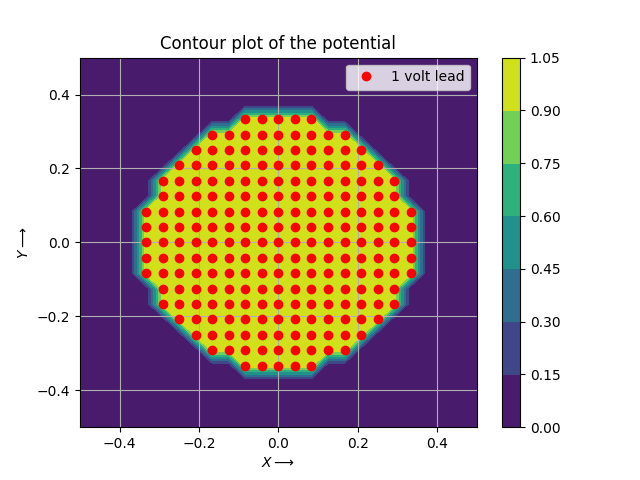
\includegraphics[scale=0.8]{contour1.png}  
        \caption{Contour plot of initial potential}
   \end{figure}
   
 \section{Updating the plate potential:}
 We will use the below equation as reference to update the potential at each point on the plate.
 Each point's potential is the average of its 4 neighbours.
   \begin{equation}
           \phi_{i,j} = \frac{\phi_{i+1,j} + \phi_{i-1,j} + \phi_{i,j+1} + \phi_{i,j-1}}{4} 
   \end{equation}
   
  We have already seen how to assign the boundary condition for each side of the plate. We will also 
  calculate the error for each iteration as,
   
   \begin{equation}
    error_k = \phi- \phi_{old}
   \end{equation}
   where $error_k$ is the error for the $k^{th}$ iteration. We will use Vectorised code to do the iterations.\newline
    \textit{\textbf{Python Code:}}
    \lstset{language=Python}
    \lstset{label={lst:code_direct}}
    \lstset{basicstyle=\footnotesize}
    \begin{lstlisting}
    errors=np.zeros(Niter)    #This block updates the value of potential at each point in the plate and
                              #keeps track of the error in each iteration
    for i in range(Niter):
        oldphi= phi.copy()
        phi[1:-1,1:-1]= 0.25*(phi[1:-1,0:-2]+phi[1:-1,2:]+phi[0:-2,1:-1]+phi[2:,1:-1])
        phi[1:-1,0]= phi[1:-1,1] 
        phi[1:-1,-1]= phi[1:-1,-2] 
        phi[0,:]= phi[1,:] 
        phi[ii]= 1.0
        errors[i]= (abs(oldphi-phi)).max()
    \end{lstlisting}


 
\section{Analysing the errors:}
  Using the error obtained by running the above code, we plot semilog and log-log plots for analysis.
  For better visualization, we plot every $50^{th}$ point. \newline The plots are given below. 
      \begin{figure}[!tbh]
      \centering
      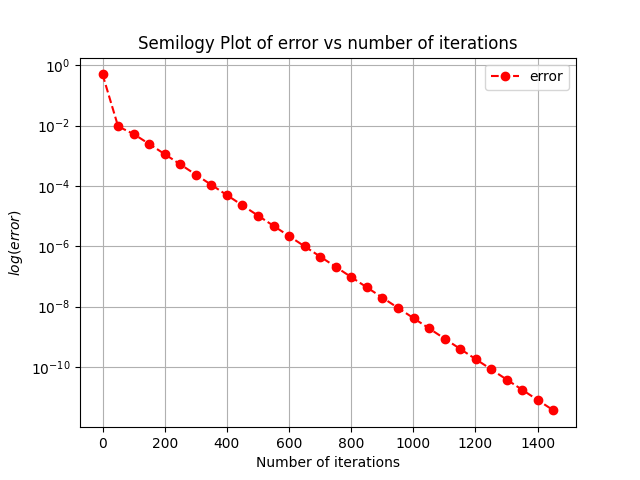
\includegraphics[scale=0.8]{semilog1.png}  
      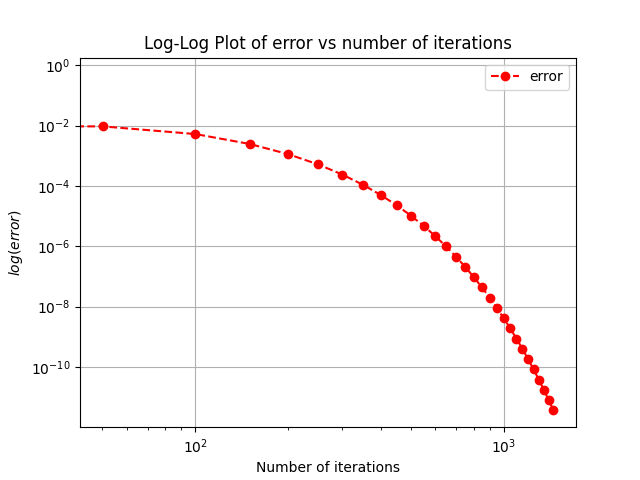
\includegraphics[scale=0.8]{loglog.png}  
      \caption{Semilog and Log-Log plots of Error vs No.of Iterations}
      \end{figure}
 \begin{itemize}
 \item
   As we observe the semilog plot that error decreases linearly for higher
   no of iterations,so from this we conclude that for large iterations
   error decreases exponentially with No of iterations i.e it follows
   \(Ae^{Bx}\) as it is a semilog plot
 \item
   And if we observe loglog plot the error is almost linearly decreasing
   for smaller no of iterations so it follows \(a^x\) form since it is
   loglog plot and follows some other pattern at larger iterations.
 \item
   So to conclude the error follows \(Ae^{Bx}\) for higher no of
   iterations(\(\approx\) 500) and it follows \(a^x\) form for smaller
   iterations which can be seen from the plots given above.
 \end{itemize}
 
\section{Least Squares Fit:}

$\rightarrow$To find the fit using Least squares for all iterations named as
  \textbf{fit1} and for iterations greater than 500 named as \textbf{fit2}
  separately and compare them.

 $\rightarrow$ As we know that error follows \(Ae^{Bx}\) at large iterations, we use
  equation given below to fit the errors using least squares

\begin{equation}
    logy = logA + Bx
\end{equation}
where A and B are constants.\newline
We can arrive at the fit for the default values as,
\begin{itemize}
\item  
Fit1 : A = 0.026628934257051245 , B = -0.01564482721966434
\item
Fit2 : A = 0.026454455729215034 , B = -0.01563763735036898
\end{itemize}
\begin{figure}[!tbh]
 \centering
 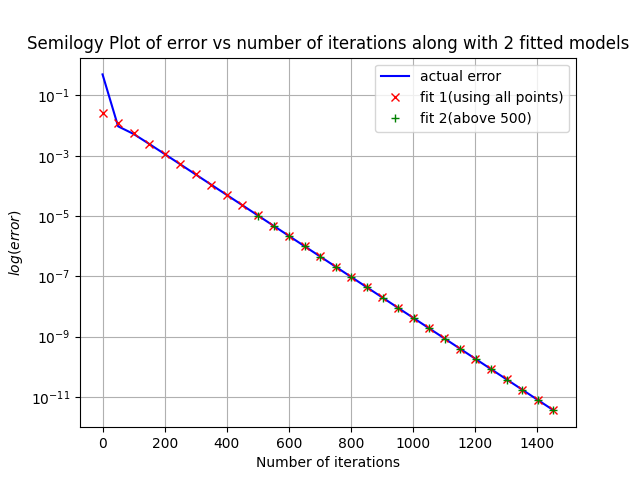
\includegraphics[scale=0.8]{semilog2.png}  
 \caption{Semilog plot of Error vs No.of Iterations}
\end{figure}

\section{Surface and Contour Plot of the Potential}
Let us plot the 3-D surface plot and the contour plot of the potential after updating its values all
over the plate.\newline

\begin{figure}[!tbh]
 \centering
 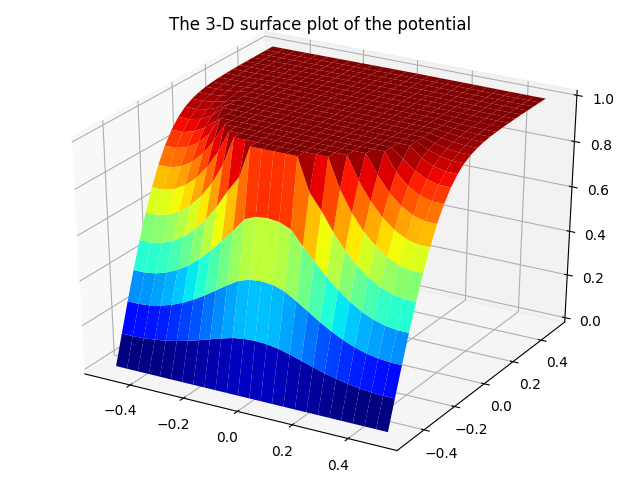
\includegraphics[scale=0.8]{surface.png}  
 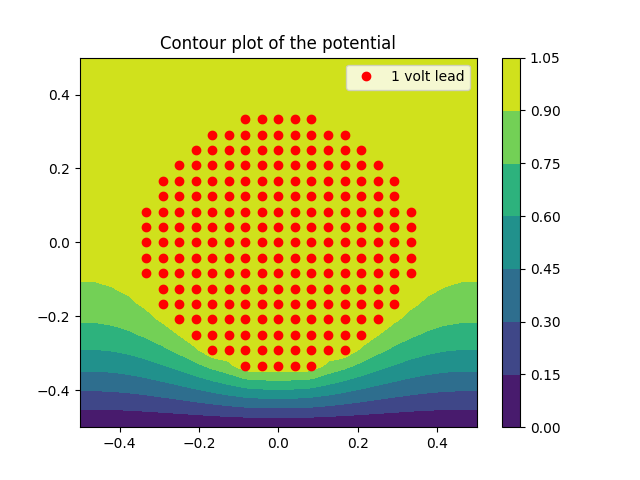
\includegraphics[scale=0.8]{contour2.png}  
 \caption{3-D Surface potential plot and Contour plot of potential}
\end{figure}

$\rightarrow$  As we observe that the surface plot we conclude that after updating
  the potential,the potential gradient is higher in down part of the
  plate since, the down side is grounded and the electrode is at 1 V,so
  there is high potential gradient from electrode to grounded plate.
\newline
$\rightarrow$  And the upper part of the plate is almost 1 V since they didnt have
  forced Voltage and their's were floating,so while applying updating we
  replaced all points by average of surrounding points so the potential
  is almost 1 V in the upper region of the plate.
\newline
$\rightarrow$ Same observation we see using contour plot in 2 dimensions, we note
  that there are gradients in down part of the plate and almost
  negligible gradient in upper part of the plate.
  \newline  The plots are given below.
\clearpage

\section{Vector Plot of Currents:}
We now further plot the current, which can be obtained simply by taking the
gradient of the potential in both the directions as per the following equation:
\begin{equation}
    J_x = -\frac{\partial \phi}{\partial x} 
  \end{equation}
\begin{equation}
    J_y = -\frac{\partial \phi}{\partial y} 
  \end{equation}
We calculate this in our program as per the following equations:
\begin{equation}
        J_{x,ij} = \frac{1}{2}(\phi_{i,j-1} - \phi_{i,j+1}) 
    \end{equation}
\begin{equation}
        J_{y,ij} = \frac{1}{2}(\phi_{i-1,j} - \phi_{i+1,j}) 
    \end{equation}
We plot the vector currents of the potential using the \texttt{quiver()} plot. The plot is given below.
  \begin{figure}[!tbh]
   \centering
   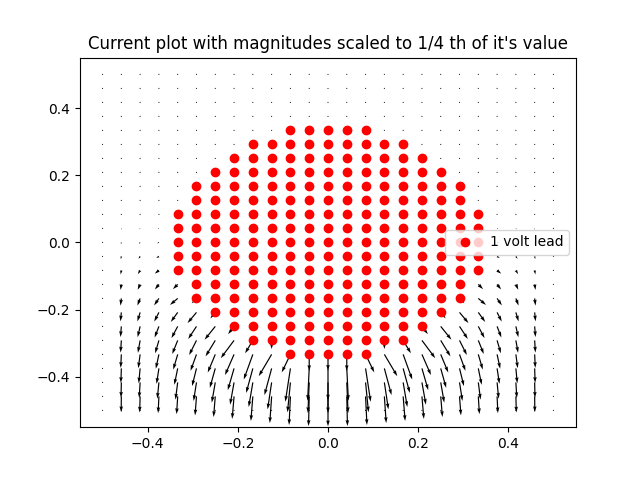
\includegraphics[scale=0.8]{current.png}  
   \caption{Vector plot of current flow}
  \end{figure}

We can very well see that the current is high in the bottom region, close to the grounded side.
This occurs because the current is directly proportional to the gradient of the potential, which is high in the bottom part.
  \begin{equation}
  \vec{E} = -\nabla{\phi}
     \end{equation}
  \begin{equation}
  \vec{J} = \sigma\vec{E}
     \end{equation}
  \begin{itemize}
  \item
    So \(\vec{J}\) is higher and perpendicular to equipotential electrode
    region i.e "Red dotted region" so the current is larger in down part
    of the plate and perpendicular to the red dotted electrode region
    since \(I\) = \(\vec{J}.\vec{A}\)
  \item
    So because of this most of the current flows from electrode to the
    bottom plate which is grounded because of higher potential gradient.
  \item
    And there is almost zero current in upper part of the plate since
    there is not much potential gradient as we observed from the surface
    and contour plot of the potential \(\phi\)
  \end{itemize}
  \section{Visualizing the Temperature with plots:}
       We know that heat generated is from \(\vec{J}.\vec{E}\) (ohmic
    loss) so since \(\vec{J}\) and \(\vec{E}\) are higher in the bottom
    region of the plate, there will more heat generation and temperature
    rise will be present.\newline
    The variation of temperature in the plate can be seen in the below 3-D surface plot. 
      \begin{figure}[!tbh]
   \centering
   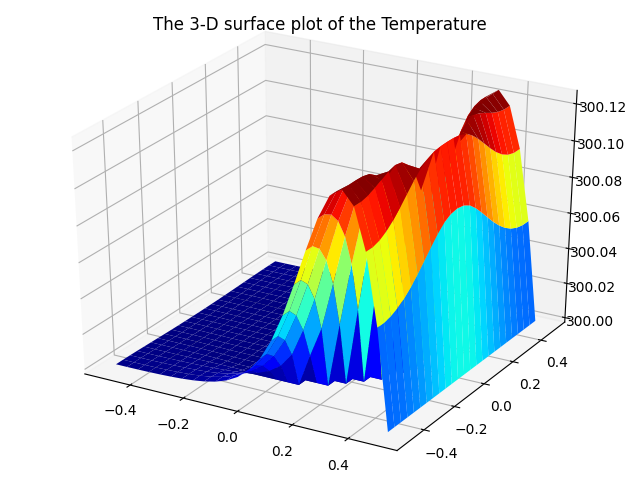
\includegraphics[scale=0.8]{surface2.png}  
   \caption{Variation of temperature in the plate}
  \end{figure}
\section{Conclusion :}
  
  \begin{enumerate}
  \item
    We have seen that most of the current is in the narrow region at the
    bottom. So that portion of the plate is what will get strongly heated.
  \item
    Since there is almost no current in the upper region of plate,the
    bottom part of the plate gets hotter and temperature increases in down
    region of the plate.
  \item
    And we know that heat generated is from \(\vec{J}.\vec{E}\) (ohmic
    loss) so since \(\vec{J}\) and \(\vec{E}\) are higher in the bottom
    region of the plate, there will more heat generation and temperature
    rise will be present.
  \item
    We saw how currents can be modelled using python in this assignment. 
  \item
    With the increase in $N_x$ and $N_y$, the contour plots become smoother as there are more number of points, thereby, getting a better circular picture for the wire.  
  \end{enumerate}
  \end{document}
